%\section{Using the MMB}
This section introduces the menu of models, policy rules and options, which can be selected in the MMB 3.1.
% For the time being, this version of the MMB does not feature the option of  model-specific shocks, and does not allow for flexible selection of the states and gain parameters used in the simulations of adaptive learning models. We will reintroduce these features into the MMB in the next release. 
\subsection*{Models}
For the time being there are some models, which cannot be simulated with Octave 4.4.0. The list of models contains: EA\_Q14. We will address these issues in the next release.

The user can select from the number of models displayed in the frontend, and from the number of policy rules. In contrast to earlier versions, the MMB 3.1 simultaneously allows for the selection of more than one policy rule and more than one model (the earlier versions either only allowed for one model, many rules or one rule, many models).  So, the user can select policy rules, shocks and variables, which are common in all selected models or remove common variables, which are automatically selected.

%\begin{figure}[H]
%	\centering
%	\caption{\textsc{Models and Rules Menu}}
%	\vspace{0.2cm}
%	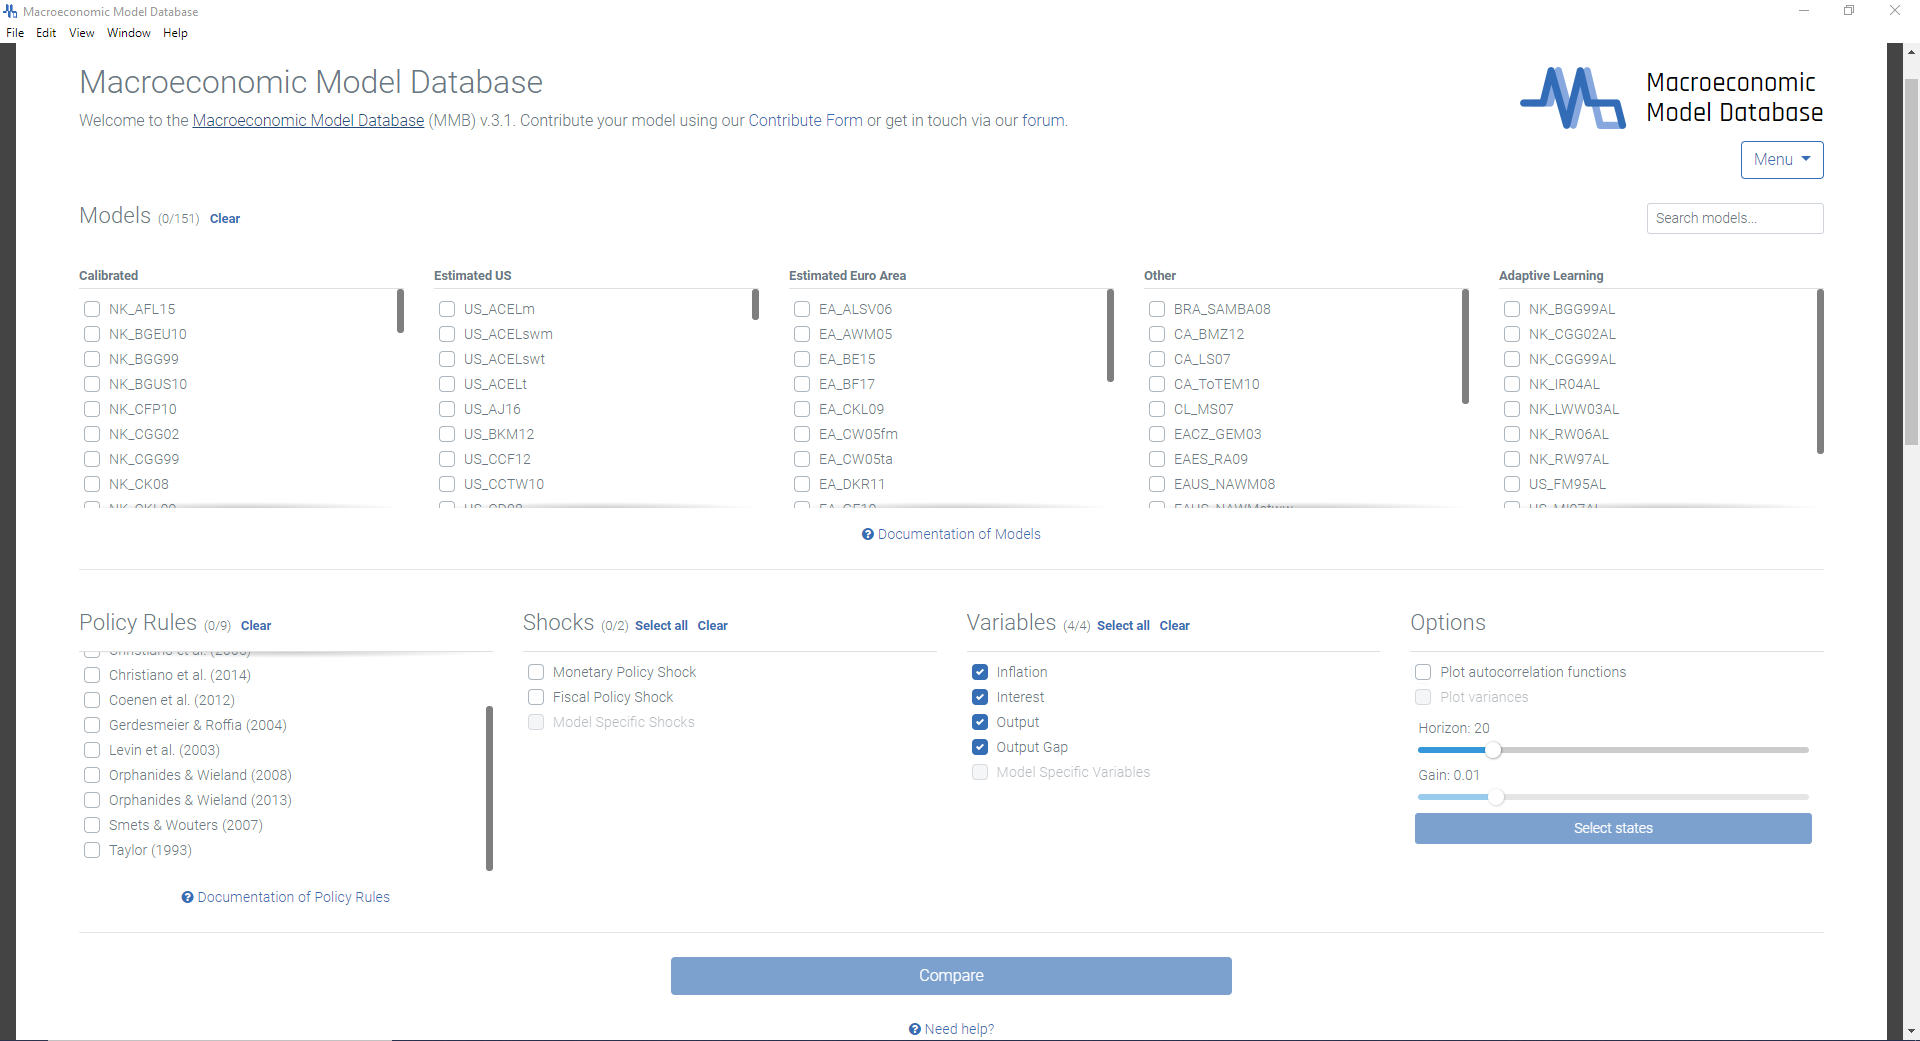
\includegraphics[width=15cm,keepaspectratio]{frontend.png}\\
%	\label{img:Models}
%\end{figure}

\begin{figure}[H]
	\centering
	\caption{\textsc{Models Menu}}
	\vspace{0.2cm}
	\includegraphics[width=15cm,keepaspectratio]{frontend_models31.png}\\
	\label{img:Models}
\end{figure}

The models are sorted in columns, the first of which contains models that have been calibrated to match a closed economy (NK\_xxx). The second column lists models that have been estimated on US data (US\_xxx). The third column lists models that have been estimated on Euro area data (EA\_xxx). The column 'Other' contains models that have been either calibrated or estimated on multi-country data, or have been estimated on other countries, such as 'CA\_BMZ12', which has been estimated on Canadian data, or 'EAUS\_NAWM08', which has been estimated on Euro area and US data in a two-economy-setting. The last column contains models in which agents form their expectations via adaptive learning (xxxAL). 
%\textbf{For the time being, until the options for the adaptive learning models are reintroduced into the MMB, all states are selected by default and the gain parameter is fixed to 0.01}. 


Hovering with the mouse over the models in the list and over the common policy rules displays some basic information such as the title, author and academic reference of the article, in which the model was used. To search for models in the MMB, one can also use the search line on top of the menu. Here one can search for the name of the author or words that appear in the title of the articles, in which the models were used as well as journals or year of publication. For instance, searching for Gal{\'\i}, yields the results shown in Figure \ref{search}.

\begin{figure}[H]
	\centering
	\caption{\textsc{Models Search: Gal{\'\i}}}
	\vspace{0.2cm}
	\includegraphics[width=15cm,keepaspectratio]{gali.png}\\
	\label{search}
\end{figure}

In addition, the user can download a complete list of all models currently used in the MMB on \url{macromodelbase.com/downloads}. Lastly, short descriptions of the models and their features are available on the same page. The menu of the MMB contains a direkt link to the model descriptions below the model selection menu as shown in Figure \ref{docmod}.
\begin{figure}[H]
	\centering
	\caption{\textsc{Model Documentation}}
	\vspace{0.2cm}
	\includegraphics[width=15cm,keepaspectratio]{documentmodels31.png}\\
	\label{docmod}
\end{figure}

\subsection*{Monetary policy rules}



Currently, we consider nine monetary policy rules that are taken from \cite{Taylor1993}, \cite{LevinWielandWilliams2003}, \cite{SmetsWouters2007}, among others. Next to these common rules that can (in principle) be used for all models, the selection menu also features the options model specific rule and user-specific rule. 
The model specific rules are taken from the original articles, in which the models were used. Not all models can be simulated with their model-specific rule, as all interest rate rules that can be used in the modelbase, have to be expressed in terms of the common variables. These common variables are the quarterly output gap, quarterly output, the year-on-year rate of inflation and the policy interest rate in annual terms. As some of the interest rate rules used in the literature feature responses to financial indicators, exchange rates, etc. these rules cannot be included in the modelbase. Therefore only 93 of the 128 models included in the MMB 3.0 feature a model-specific rule. 
%%%%%%%%%%%%%%%%%%%%%
%CHECK THESE NUMBERS%
%%%%%%%%%%%%%%%%%%%%%

\begin{figure}[H]
	\centering
	\caption{\textsc{Policy Rules Menu}}
	\vspace{0.2cm}
	\includegraphics[width=15cm,keepaspectratio]{frontend_pr31.png}\\
	\label{img:PR}
\end{figure}

The user specific rule allows the user to directly determine the feedback coefficients in the interest rate rule. In order to do so, the user has to click on `(edit)' next to the entry `User specific rule' as shown in figure \ref{img:PR}. Then, the subwindow shown in figure \ref{userrule} opens. In this example, the coefficients for current and lagged inflation rates, as well as for the current output gap are chosen such as to mimic the pre-programmed Taylor rule. The time indices refer to quarters. Click on `OK' to set the policy rule or on `Cancel' to discard changes.

The user can edit the coefficients of the responses of the policy rates to the leads and lags of the variables in this submenu. However, it is not guaranteed that the Blanchard-Kahn conditions will hold and a determined equilibrium is obtained in the solution of the models with this rule. 

\begin{figure}[H]
	\centering
	\caption{\textsc{Model Documentation}}
	\vspace{0.2cm}
	\includegraphics[width=15cm,keepaspectratio]{userrule.png}\\
	\label{userrule}
\end{figure}

In general, when a model (or a pre-specified rule) is chosen that is not compatible with a policy rule (or a model) in the way that a simulation of this model-rule-combination does not render the rational expectation equilibrium locally unique, the respective policy rule (or model) is faded out in the menu and cannot be selected for the comparison exercise. Unselecting the model (or rule), makes the rule (or model) again accessible for selection. 

\subsection*{Output options}

Having chosen the models and a policy rule, the user can make some non-exclusive choices regarding the exercise outcomes to be displayed.
The user can decide whether to see the unconditional variances and plot autocorrelation functions of the common variables, both of which are computed using theoretical moments of the solution for each variable. Also the user can opt for plotting impulse response functions of the common variables and specify the horizon for the analysis that is set to twenty periods as a default. 

As default the common MMB variables (quarterly output gap, quarterly output, the year-on-year rate of inflation and the policy interest rate in annual terms) are selected. If only one model is chosen, all other variables as defined in the mod-file are also available. As a new feature in the MMB 3.1, some more variables which are featured in many of the models, but not in all of them  (among others consumption, investment and capital) can be selected for comparison if available in all selected models. 

One can choose impulse responses to a unit monetary policy shock (one percent point increase in the monetary policy shock), and/or to a unit fiscal policy shock (one percent increase in GDP share of government expenditures). Note that all models of the Modelbase have a monetary policy shock, but a significant number of them do not have a fiscal policy shock. If this is the case, the impulse responses to a fiscal policy shock will not be available. Again, if only one model is selected, all model-specific shocks as defined in the mod-file are available for selection. Alongside the new comparable variables, also a number of shocks  appearing in many models are now available for comparison (e.g. Technology shock, Preference shock).
%AL

When you select an adaptive learning model, you can also set the gain parameter and select the states by clicking on `Select states'. In the window that pops up you can select the states individually for all adaptive learning models you have selected for the comparison.

Lastly, for certain models, the unconditional variances are not defined and the autocorrelation functions do not exist. This is the case for some models which feature unit roots. The presence of unit roots prevents a calculation of unconditional moments of some or all variables. Nonetheless, for these models IRFs can still be generated. 


\subsection*{Menu}
In the upper right corner of the MMB GUI you can find the button `Menu'. When clicking the button, a drop-down menu opens, where you can click four buttons.\\
Firstly, `Edit Rules/Models' opens a sub-window with all models included in the MMB. Here you can manually find the model you want to edit. After clicking on a model name, you can see its two relevant files, namely the .json and .mod file. The .json file contains basic information about the model, like paper title, author and journal, but it also contains information about the model capabilities, i.e. if the model is capable of producing the common variables (output, inflation, interest rate, output gap) and common shock (monetary and fiscal policy shock). As an example, \textit{fiscal\_shock": false} means that the model does not contain a fiscal policy shock. You can also see if unconditional variances are possible for this model and if it is an adaptive learning model. Furthermore, under \textit{rules} you can see which policy rule is eligible for the model you want to edit, while under \textit{msr} you can see and change the coefficients for the model specific policy rule. In the block below, you can see the name and the text of each shock and below that of each variable contained in the model. In case you want to change the name of a shock or variable appearing in the main-window, please change its text to the desired text. Hint: The text is case sensitive, so if you want to change the name of a variable for many models, be consistent with the text. The other file appearing in for the selected model is the .mod file. This file consists of a preamble defining all variables, shocks and parameters. It is followed by the parameter initialization and the model equations, which define the sticky price and wage economy and the flex economy, as well as shocks. In the case of non-zero steady state values of variables, there usually also exists a separate \textit{modelname\_steadystate.m} file, which defines the steady state of the model. In the upper right corner of the sub-window you can save the changes of the current file. It is important to keep in mind that you need to save the file before switching to another file because then unsaved changes are gone. Also, saving the changes does not apply them. You need to reload the data. At any time you can close the sub-window by clicking the `Close' button in the lower right corner of the sub-window. 
%There is no folder with policy rules, only models

The second button in the drop-down menu is `Reload Data' and applies the saved changes made to the files, i.e. renaming a shock or variable.
%%%%%%%%%%%%%%%%%%%%%%%%%%%%%%%%%%%%
%Maybe problem here (when renaming)%  
%%%%%%%%%%%%%%%%%%%%%%%%%%%%%%%%%%%%

The third button `Settings' is explained in section \ref{sec:installation}.

The last button `Help' opens a help window. 


\subsection*{Running a comparison exercise}
Once you have selected a number of models, rules and output options, you can simply run the comparison exercise by clicking on the button `Compare'. When the simulations run the command window from MATLAB/OCTAVE will be embedded and you see the running output (see, Figure \ref{mmbsimul}). Once the simulations are finished you can close the window by clicking on `Close'.
%If you have chosen to run your simulations using OCTAVE, the command window from OCTAVE will be embedded and you see the running output (see, Figure \ref{mmbsimul}). If you are using MATLAB, a second window opens, in which the simulations are displayed as in MATLAB's command window. This second window closes automatically when the simulations are done.
 
\begin{figure}[H]
	\centering
	\caption{\textsc{Model Simulation}}
	\vspace{0.2cm}
	\includegraphics[width=15cm,keepaspectratio]{mmbsimul.png}\\
	\label{mmbsimul}
\end{figure}

As a result, the selected Impulse response functions and  autocorrelation functions are plotted, and the variances are displayed in a table at the bottom of the frontend. 
There are different options available to display the results (see figure \ref{display}). First, the user can choose whether results should be displayed in charts of variables, models or policy rules. This can be selected by clicking on `Group Data' and then the respective option. The default is to group outputs by variable, i.e. the charts represent variables and the graphs in the charts represent model/policy rule-combinations. 
Further, the user can select the `maximum number of columns per row', which might be useful to increase readability or clarity depending on the screen used. 
Finally, the user can choose which graphs are displayed in the charts by clicking on the respective entries of the caption.

\begin{figure}[H]
	\centering
	\caption{\textsc{Display Options}}
	\vspace{0.2cm}
	\includegraphics[width=15cm,keepaspectratio]{display31.png}\\
	\label{display}
\end{figure}


The results of the comparison exercise can be exported and saved in two ways. Either, one exports all the data, by clicking on CSV or JSON above the figures to receive a batch export in the respective file format, or one can export the figures one by one, by clicking on the menu on the upper right corner of each figure. Both options are marked with red boxes in Figure \ref{export}.
\begin{figure}[H]
	\centering
	\caption{\textsc{Export Options}}
	\vspace{0.2cm}
	\includegraphics[width=15cm,keepaspectratio]{export.png}\\
	\label{export}
\end{figure}
